\documentclass[tikz,border=6pt]{standalone}
\usepackage[sfdefault,lining]{FiraSans}
\usepackage{amsmath}
\usepackage{firamath-otf}
\setmathrm{Fira Sans}
\usepackage{pgfplots}
\pgfplotsset{compat=1.18}
\usetikzlibrary{arrows.meta,calc,patterns}
\definecolor{ink}{HTML}{1F2A37}\definecolor{grey}{HTML}{6B7280}\definecolor{sea}{HTML}{1D4E89}
\definecolor{accent}{HTML}{0F766E}
\newcommand{\wavecol}[2]{\definecolor{tmpwave}{wave}{#2}\colorlet{#1}[rgb]{tmpwave}}
\begin{document}

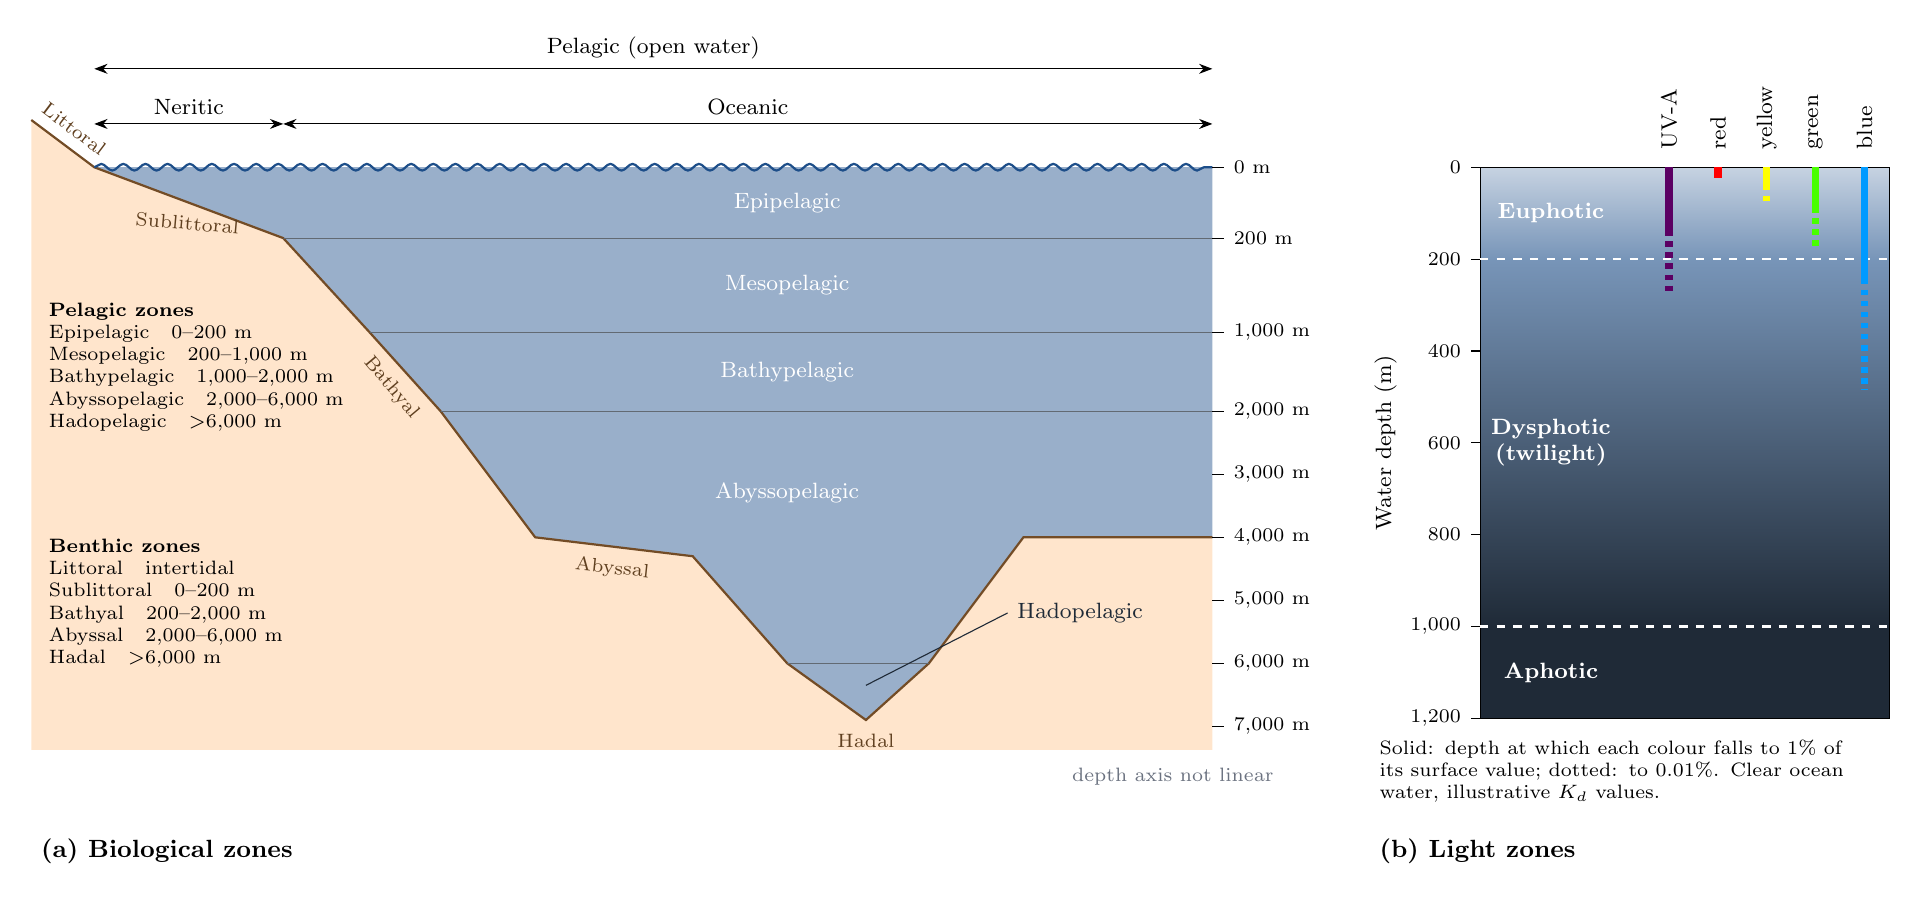
\begin{tikzpicture}[font=\small]
\fill[sea!45] (0.8,0.000) -- (3.2,-0.900) -- (4.3,-2.100) -- (5.2,-3.100) -- (6.4,-4.700) -- (8.4,-4.940) -- (9.6,-6.300) -- (10.6,-7.020) -- (11.4,-6.300) -- (12.6,-4.700) -- (15,-4.700) -- (15,0) -- cycle;
\fill[orange!20] (0,0.6) -- (0.8,0.000) -- (3.2,-0.900) -- (4.3,-2.100) -- (5.2,-3.100) -- (6.4,-4.700) -- (8.4,-4.940) -- (9.6,-6.300) -- (10.6,-7.020) -- (11.4,-6.300) -- (12.6,-4.700) -- (15,-4.700) -- (15,-7.4) -- (0,-7.4) -- cycle;
\draw[thick,brown!60!black] (0,0.6) -- (0.8,0.000) -- (3.2,-0.900) -- (4.3,-2.100) -- (5.2,-3.100) -- (6.4,-4.700) -- (8.4,-4.940) -- (9.6,-6.300) -- (10.6,-7.020) -- (11.4,-6.300) -- (12.6,-4.700) -- (15,-4.700);
\draw[sea,thick,decorate,decoration={snake,amplitude=1.2pt,segment length=8pt}] (0.8,0) -- (15,0);
\begin{scope}\clip (0.8,0.000) -- (3.2,-0.900) -- (4.3,-2.100) -- (5.2,-3.100) -- (6.4,-4.700) -- (8.4,-4.940) -- (9.6,-6.300) -- (10.6,-7.020) -- (11.4,-6.300) -- (12.6,-4.700) -- (15,-4.700) -- (15,0) -- cycle;
\draw[ink!70] (0,-0.900) -- (15,-0.900);
\draw[ink!70] (0,-2.100) -- (15,-2.100);
\draw[ink!70] (0,-3.100) -- (15,-3.100);
\draw[ink!70] (0,-6.300) -- (15,-6.300);
\end{scope}
\node[font=\footnotesize,white] at (9.6,-0.450) {Epipelagic};
\node[font=\footnotesize,white] at (9.6,-1.500) {Mesopelagic};
\node[font=\footnotesize,white] at (9.6,-2.600) {Bathypelagic};
\node[font=\footnotesize,white] at (9.6,-4.140) {Abyssopelagic};
\draw[ink] (10.6,-6.580) -- (12.4,-5.660) node[right,font=\footnotesize,ink] {Hadopelagic};
\draw (15,0.000) -- (15.15,0.000) node[right,font=\scriptsize] {0 m};
\draw (15,-0.900) -- (15.15,-0.900) node[right,font=\scriptsize] {200 m};
\draw (15,-2.100) -- (15.15,-2.100) node[right,font=\scriptsize] {1,000 m};
\draw (15,-3.100) -- (15.15,-3.100) node[right,font=\scriptsize] {2,000 m};
\draw (15,-3.900) -- (15.15,-3.900) node[right,font=\scriptsize] {3,000 m};
\draw (15,-4.700) -- (15.15,-4.700) node[right,font=\scriptsize] {4,000 m};
\draw (15,-5.500) -- (15.15,-5.500) node[right,font=\scriptsize] {5,000 m};
\draw (15,-6.300) -- (15.15,-6.300) node[right,font=\scriptsize] {6,000 m};
\draw (15,-7.100) -- (15.15,-7.100) node[right,font=\scriptsize] {7,000 m};
\node[font=\scriptsize,grey,anchor=north east] at (15.9,-7.5) {depth axis not linear};
\node[rotate=-5,font=\scriptsize,brown!50!black,anchor=north] at (2.0,-0.500) {Sublittoral};
\node[rotate=-50,font=\scriptsize,brown!50!black,anchor=north] at (4.75,-2.650) {Bathyal};
\node[rotate=-6,font=\scriptsize,brown!50!black,anchor=north] at (7.4,-4.870) {Abyssal};
\node[rotate=0,font=\scriptsize,brown!50!black,anchor=north] at (10.6,-7.070) {Hadal};
\node[rotate=-37,font=\scriptsize,brown!50!black,anchor=south] at (0.42,0.32) {Littoral};
\draw[{Stealth}-{Stealth}] (0.8,0.55) -- node[above,font=\footnotesize] {Neritic} (3.2,0.55);
\draw[{Stealth}-{Stealth}] (3.2,0.55) -- node[above,font=\footnotesize] {Oceanic} (15,0.55);
\draw[{Stealth}-{Stealth}] (0.8,1.25) -- node[above,font=\footnotesize] {Pelagic (open water)} (15,1.25);
\node[anchor=north west,font=\scriptsize,align=left] at (0.1,-1.6) {\textbf{Pelagic zones}\\Epipelagic\quad 0--200 m\\Mesopelagic\quad 200--1,000 m\\Bathypelagic\quad 1,000--2,000 m\\Abyssopelagic\quad 2,000--6,000 m\\Hadopelagic\quad $>$6,000 m};
\node[anchor=north west,font=\scriptsize,align=left] at (0.1,-4.6) {\textbf{Benthic zones}\\Littoral\quad intertidal\\Sublittoral\quad 0--200 m\\Bathyal\quad 200--2,000 m\\Abyssal\quad 2,000--6,000 m\\Hadal\quad $>$6,000 m};
\node[anchor=north west,font=\small\bfseries] at (0,-8.4) {(a) Biological zones};
\shade[top color=sea!25,bottom color=sea!60] (18.4,0) rectangle (23.599999999999998,-1.1666666666666665);
\shade[top color=sea!60,bottom color=ink] (18.4,-1.1666666666666665) rectangle (23.599999999999998,-5.833333333333334);
\fill[ink] (18.4,-5.833333333333334) rectangle (23.599999999999998,-7.0);
\draw (18.4,0) rectangle (23.599999999999998,-7.0);
\draw[dashed,white,thick] (18.4,-1.1666666666666665) -- (23.599999999999998,-1.1666666666666665);
\draw[dashed,white,thick] (18.4,-5.833333333333334) -- (23.599999999999998,-5.833333333333334);
\draw (18.4,0.0) -- (18.279999999999998,0.0) node[left,font=\scriptsize] {0};
\draw (18.4,-1.1666666666666665) -- (18.279999999999998,-1.1666666666666665) node[left,font=\scriptsize] {200};
\draw (18.4,-2.333333333333333) -- (18.279999999999998,-2.333333333333333) node[left,font=\scriptsize] {400};
\draw (18.4,-3.5) -- (18.279999999999998,-3.5) node[left,font=\scriptsize] {600};
\draw (18.4,-4.666666666666666) -- (18.279999999999998,-4.666666666666666) node[left,font=\scriptsize] {800};
\draw (18.4,-5.833333333333334) -- (18.279999999999998,-5.833333333333334) node[left,font=\scriptsize] {1,000};
\draw (18.4,-7.0) -- (18.279999999999998,-7.0) node[left,font=\scriptsize] {1,200};
\node[rotate=90,font=\footnotesize] at (17.2,-3.5) {Water depth (m)};
\node[white,font=\footnotesize\bfseries,align=center] at (19.299999999999997,-0.5833333333333333) {Euphotic};
\node[white,font=\footnotesize\bfseries,align=center] at (19.299999999999997,-3.5) {Dysphotic\\(twilight)};
\node[white,font=\footnotesize\bfseries,align=center] at (19.299999999999997,-6.416666666666666) {Aphotic};
\wavecol{lc0}{385}
\draw[lc0,line width=2.6pt] (20.799999999999997,0) -- (20.799999999999997,-0.800);
\draw[lc0,line width=2.6pt,dash pattern=on 2pt off 2pt] (20.799999999999997,-0.800) -- (20.799999999999997,-1.599);
\node[rotate=90,anchor=west,font=\footnotesize] at (20.799999999999997,0.1) {UV-A};
\wavecol{lc1}{660}
\draw[lc1,line width=2.6pt] (21.419999999999998,0) -- (21.419999999999998,-0.070);
\draw[lc1,line width=2.6pt,dash pattern=on 2pt off 2pt] (21.419999999999998,-0.070) -- (21.419999999999998,-0.141);
\node[rotate=90,anchor=west,font=\footnotesize] at (21.419999999999998,0.1) {red};
\wavecol{lc2}{580}
\draw[lc2,line width=2.6pt] (22.039999999999996,0) -- (22.039999999999996,-0.224);
\draw[lc2,line width=2.6pt,dash pattern=on 2pt off 2pt] (22.039999999999996,-0.224) -- (22.039999999999996,-0.448);
\node[rotate=90,anchor=west,font=\footnotesize] at (22.039999999999996,0.1) {yellow};
\wavecol{lc3}{530}
\draw[lc3,line width=2.6pt] (22.659999999999997,0) -- (22.659999999999997,-0.507);
\draw[lc3,line width=2.6pt,dash pattern=on 2pt off 2pt] (22.659999999999997,-0.507) -- (22.659999999999997,-1.014);
\node[rotate=90,anchor=west,font=\footnotesize] at (22.659999999999997,0.1) {green};
\wavecol{lc4}{470}
\draw[lc4,line width=2.6pt] (23.279999999999998,0) -- (23.279999999999998,-1.414);
\draw[lc4,line width=2.6pt,dash pattern=on 2pt off 2pt] (23.279999999999998,-1.414) -- (23.279999999999998,-2.828);
\node[rotate=90,anchor=west,font=\footnotesize] at (23.279999999999998,0.1) {blue};
\node[anchor=north west,font=\scriptsize,align=left,text width=6.3cm] at (17.0,-7.15) {Solid: depth at which each colour falls to 1\% of its surface value; dotted: to 0.01\%. Clear ocean water, illustrative $K_d$ values.};
\node[anchor=north west,font=\small\bfseries] at (17.0,-8.4) {(b) Light zones};
\end{tikzpicture}\end{document}